\apendice{Documentación de usuario}

\section{Introducción}

En este apéndice se detallan los requisitos para acceder al proyecto por parte de un usuario. Además se han descrito las funcionalidades de la aplicación en un manual de usuario.

\section{Requisitos de usuarios}

Al ser una aplicación web únicamente es necesario tener un navegador web y acceder mediante el enlace \url{https://mixingmodels.netlify.app/}. Por otra parte si se quiere poder ver el contenido .csv, se requiere alguna herramienta de lectura de hojas de cálculo.

\section{Instalación}

No requiere ninguna instalación.

\section{Manual del usuario}

Esta sección es dedicada a un apartado de guía de usuario, orientando a las personas que utilicen la web, ofreciendo asistencias a los usuarios y recopilando todas las funcionalidades que ofrece.

\subsubsection{Menú superior}

En la parte de superior de la pantalla encontramos un menú superior \ref{fig:topnav} que organiza la web en algunos apartados:

\begin{figure}[h!] 
\centering
    
\includegraphics[width=1\textwidth]{img/menu_sup.PNG}
\caption{Top Navigation Bar}
\label{fig:topnav}
\end{figure}

\begin{enumerate}
    \item \textbf{Problema:} vista principal contiene la resolución de problemas de sistemas ecuaciones con restricciones, recepción y exportación de datos. 
    \item \textbf{Video:} vista contiene un vídeo guía, que permite ver las principales funcionalidades de la aplicación al usuario aportando un ejemplo básico de resolución.
    \item \textbf{Icono GitHub:} enlace directo al repositorio GitHub, que contiene el código de la aplicación y documentación del proyecto.
    \item \textbf{About us:} desplegable que muestra los desarrolladores del proyecto.
    \item \textbf{Select de traducciones:} seleccionable que nos permite cambiar entre los dos idiomas de la aplicación Ingles y Español, únicamente dando click en al idioma que queramos cambiar.
\end{enumerate}

\subsubsection{Ventana resolución problema}

En esta ventana vemos la barra de navegación superior, y el contenido de la aplicación. El funcionamiento de la web es que según se introducen datos y se va creando la estructura del problema a resolver, se van desbloqueando apartados, terminando el último con la solución del problema y los botones de exportar.

En la Figura \ref{fig:ventana_inicial} aparece el primer formulario de la aplicación, destinado a marcar el tamaño de la matriz de fuentes de datos. Es importante recalcar que el botón \textit{``Crear''} no se activa mientras los valores de marcadores y fuentes sean inferiores o iguales a cero. Una vez rellenemos el formulario con valores válidos se habilitara el botón. Por otra parte disponemos de un botón adicional (Figura \ref{fig:importPlant}) que permite al usuario cargar una plantilla de datos. Esta parte se comentará en profundidad más adelante analizando la plantilla que requiere la aplicación.


\begin{figure}[h!] 
\centering
    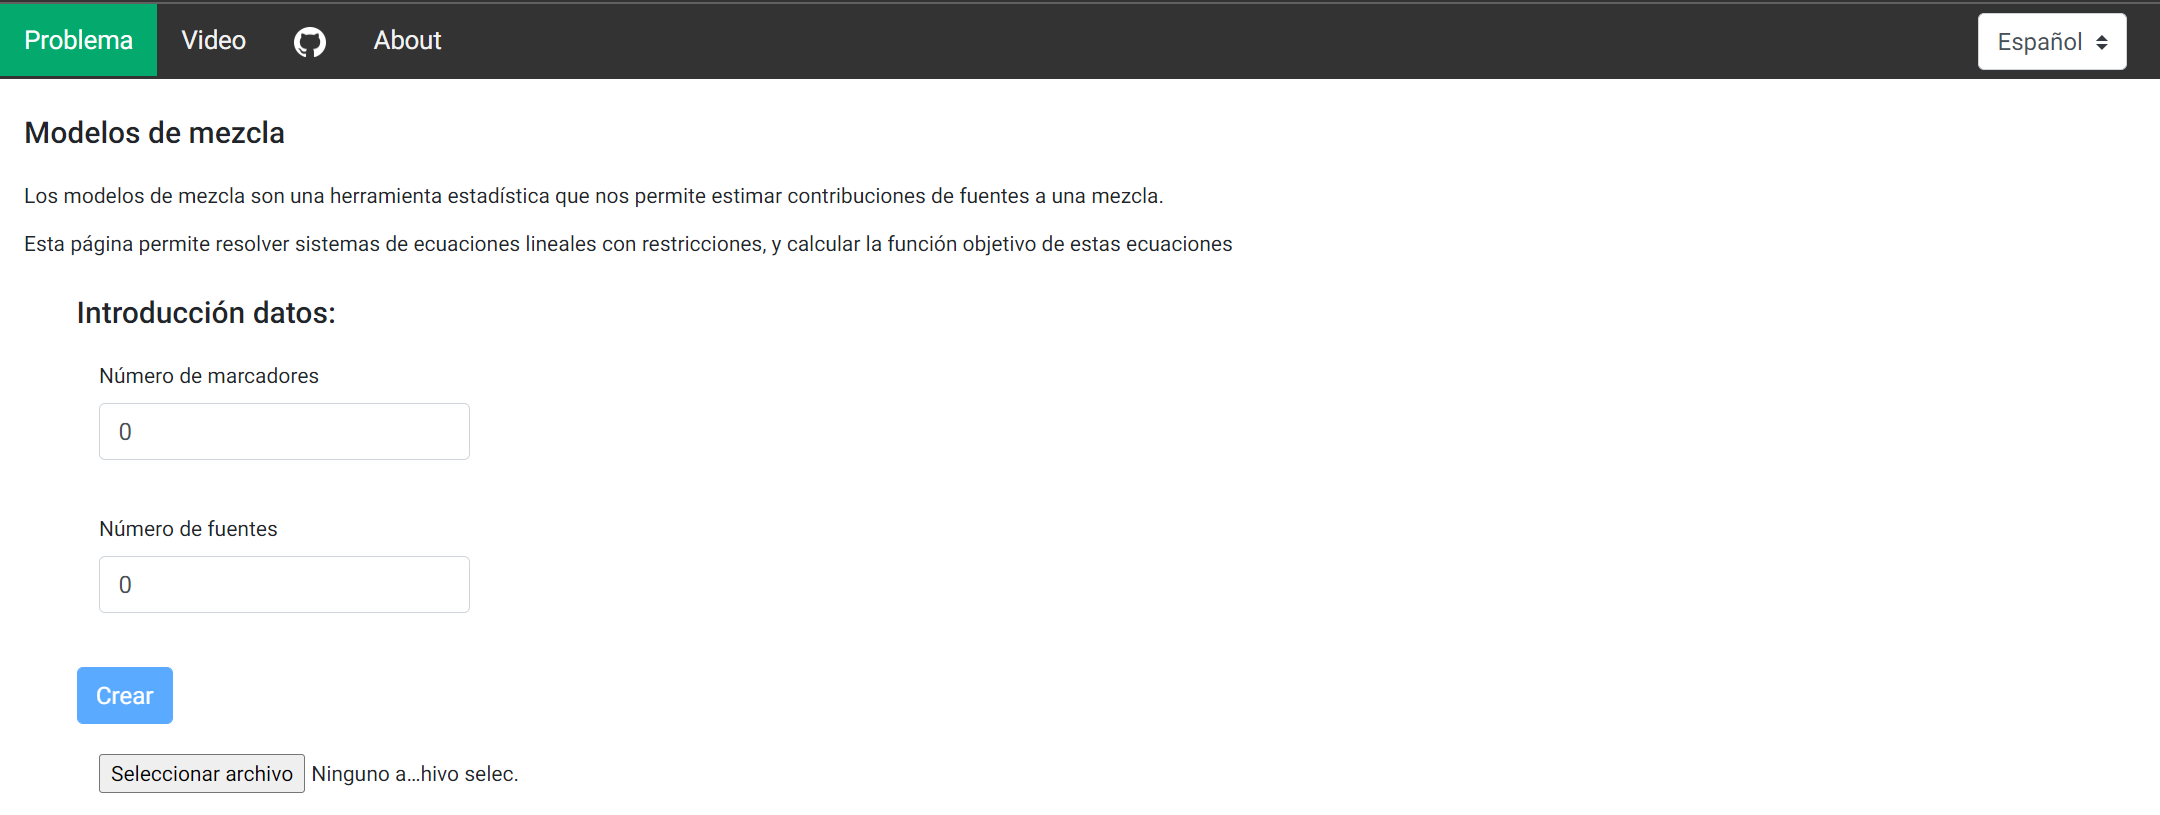
\includegraphics[width=1\textwidth]{img/ventana_inicial.PNG}
\caption{Ventana inicial web}
\label{fig:ventana_inicial}
\end{figure}

Una vez se habilita y pulsamos \textit{``Crear''}, muestra un nuevo formulario (Figura \ref{fig:data_matrix}). Siendo una matriz del tamaño fijado en el primer formulario, las filas son el número de fuentes y las columnas el número de marcadores. Se permite la introducción con números decimales, y para marcar la coma decimal se realiza con ".". Por otra parte, se ha añadido la opción de nombrar a las fuentes según queramos ofreciendo más personalización al problema.

\begin{figure}[h!] 
\centering
    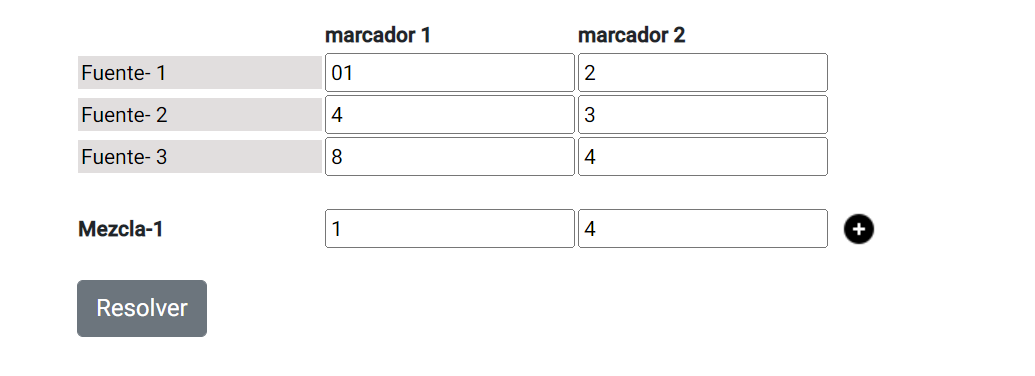
\includegraphics[width=1\textwidth]{img/datos_matriz.PNG}
\caption{Inputs datos matriz de fuentes}
\label{fig:data_matrix}
\end{figure}

En la parte inferior se encuentra la introducción de datos de las mezclas, teniendo estas el mismo número de marcadores que las fuentes. Inicialmente se encuentran datos de entrada para una única mezcla, pero podemos añadir con el botón situado a su derecha en la figura \ref{fig:data_matrix}, al pulsar, crea una nueva mezcla con el mismo tamaño de marcadores que el resto. 

Una vez hemos configurado la matriz de datos de entrada tanto de fuentes como de mezclas damos a \textit{``Resolver''}. En este momento se ejecuta una función que primero calcula las proyecciones de las mezclas respecto al plano de las fuentes y posteriormente se usa la librería GLPK para resolver el sistema. El ejercicio resuelve el sistema de ecuaciones con la restricción de que todas las $x$ cantidades deben ser superiores a $0$, esto es porque no se puede tener negativos de una cantidad. 

Por último se muestra la solución del sistema de ecuaciones mostrando las cantidades mínimas y máximas que pueden tener las fuentes respecto a las mezclas (Figura \ref{fig:sols_arrays}).

\begin{figure}[h!] 
\centering
    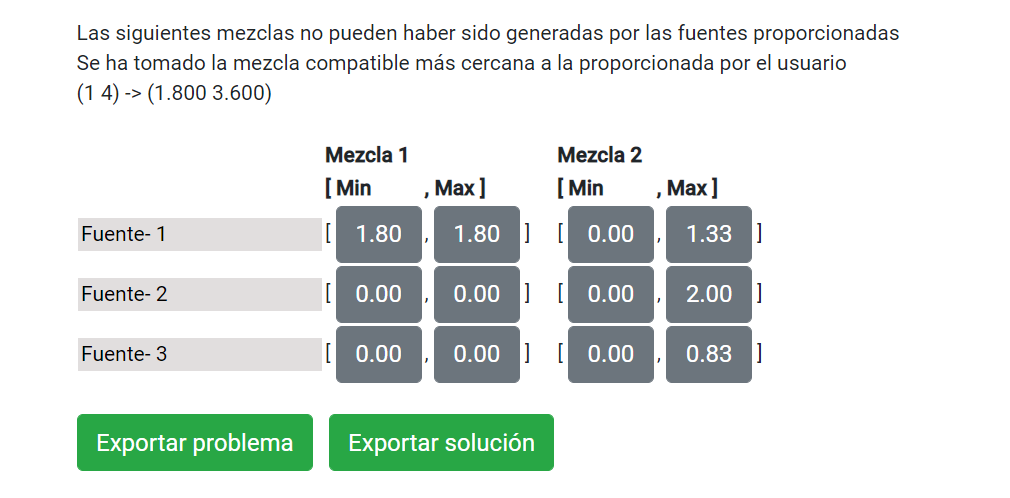
\includegraphics[width=1\textwidth]{img/solution_visual.PNG}
\caption{Arrays solución máximos y mínimos}
\label{fig:sols_arrays}
\end{figure}

En caso de que los \textit{"puntos mezclas"} se encuentre fuera del plano de fuentes, en una primera parte nos mostrará las proyecciones, las cuales son los valores utilizados en la resolución del sistema. 

Justo debajo de las proyecciones encontramos los arrays de solución de mínimos y máximos para cada mezcla sobre las fuentes. En la figura \ref{fig:sols_arrays} vemos entonces que la \textit{Fuente-1} tendría una proporción mínima de $1.80$ y una máxima de $1.80$ sobre la \textit{Mezcla 1}, y una proporción mínima de $0.00$ y una máxima de $1.33$ sobre la \textit{Mezcla 2}, comentar que estos valores solución se han redondeado a dos decimales y las proyecciones a tres.

Una vez hemos resuelto el ejercicio, la aplicación ofrece diferentes opciones de exportar los datos de la solución, a continuación veremos las tres posibilidades:

\textbf{Exportar problema: } en la figura \ref{fig:sols_arrays} si presionamos \textit{``Exportar problema''} nos descarga un archivo con nombre \textit{``InputData.csv''} que contiene los datos de la figura \ref{fig:inputData}. Manteniendo siempre la misma estructura: las dos primeras filas marcan el tamaño de la matriz de datos \textbf{marcadores} y \textbf{fuentes}, una fila en blanco y justo debajo una fila por cada fuente que se haya especificado. Por último, dejando una línea de separación encontramos una fila para cada mezcla. 

El objetivo de este documento es servir como plantilla que permita cargar este mismo problema en futuros usos.

\begin{figure}[h!] 
\centering
    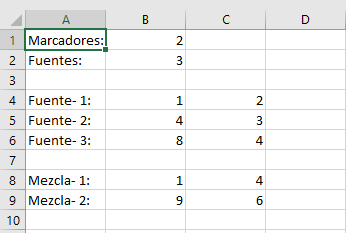
\includegraphics[width=1\textwidth]{img/inputData.PNG}
\caption{Export datos entrada problema}
\label{fig:inputData}
\end{figure}

\textbf{Exportar solución: } en la figura \ref{fig:sols_arrays} si presionamos \textit{``Exportar solución''} nos descarga un archivo de nombre \textit{"Solution.csv"}, que contiene la estructura de datos de la figura \ref{fig:solution}. El objetivo de este documento es tanto mostrar los datos de entrada como la solución del sistema, en las primeras filas encontramos el mismo diseño que con \textit{``Exportar problema''}. A continuación, se deja una línea en blanco y se muestra las proyecciones de las mezclas en caso de haberlas. Se deja otra fila en blanco y se muestra una estructura de tabla muy parecida a la visual de la web.

\begin{figure}[h!] 
\centering
    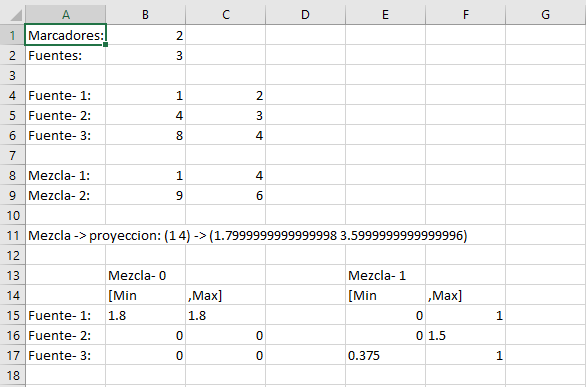
\includegraphics[width=1\textwidth]{img/solution.PNG}
\caption{Export solución completa}
\label{fig:solution}
\end{figure}

\textbf{Exportar pasos intermedios:} para descargar este documento podemos pulsar encima del número de la solución del cual queramos ver sus pasos intermedios, en el caso de la figura \ref{fig:pasoIntermedio} se ha pulsado sobre el valor $1.80$ de la \textit{Fuente-1} y \textit{Min} de la \textit{Mezcla-1}.

La estructura del documento está compuesta por unas primeras filas con restricciones del sistema, la función objetivo y las ecuaciones del sistema de ecuaciones.

\begin{figure}[h!] 
\centering
    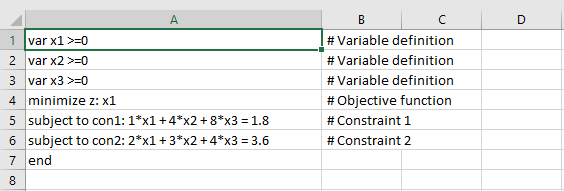
\includegraphics[width=1\textwidth]{img/pasoIntermedio.PNG}
\caption{Export resolución paso intermedio}
\label{fig:pasoIntermedio}
\end{figure}

A partir del documento de la figura \ref{fig:inputData} que funciona como plantilla de entrada podemos pulsar el botón \textit{"Seleccionar archivo"} de la figura \ref{fig:selectFile}. Esta acción abre el nuestro sistema de directorios (Figura \ref{fig:importPlant}) y podemos seleccionar la plantilla de datos exportada anteriormente. 

\begin{figure}[h!] 
\centering
    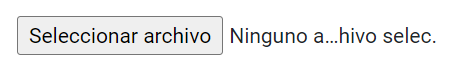
\includegraphics[width=1\textwidth]{img/selectFile.PNG}
\caption{Botón seleccionar archivo}
\label{fig:selectFile}
\end{figure}

\begin{figure}[h!] 
\centering
    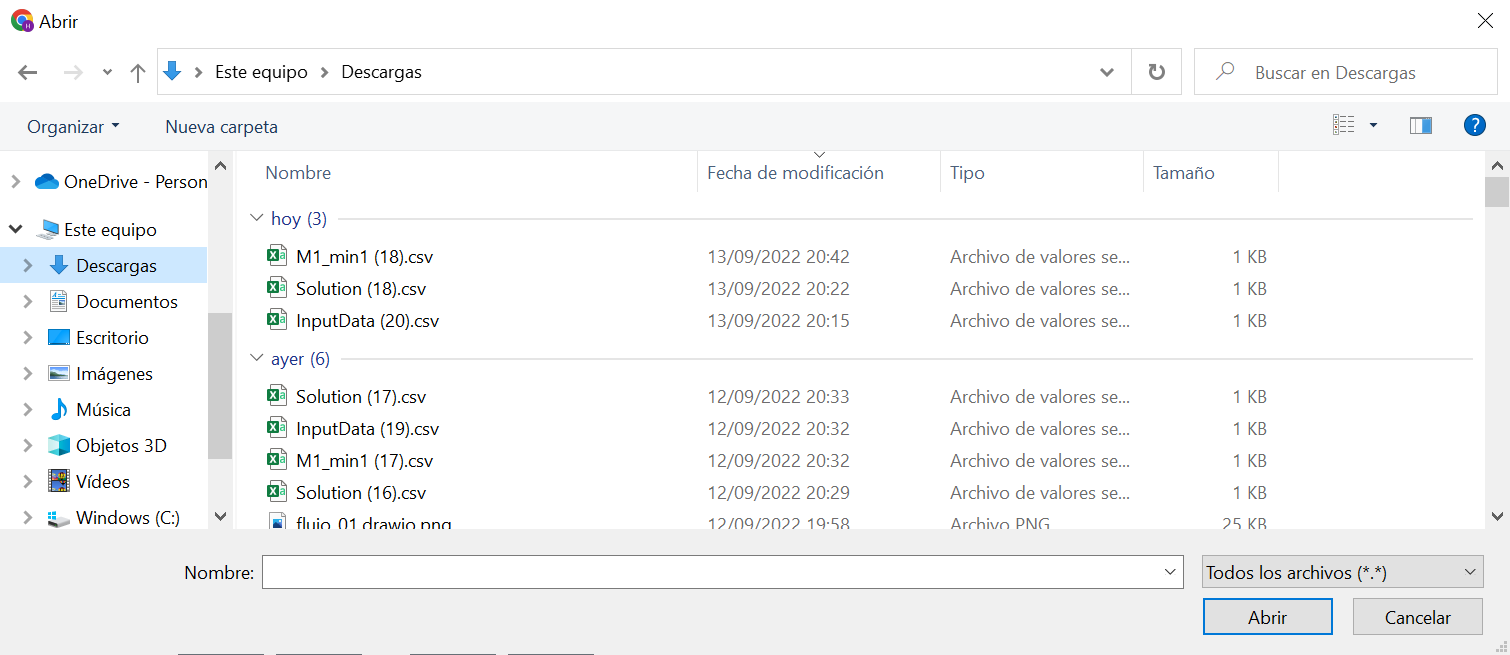
\includegraphics[width=1\textwidth]{img/directoryInport.PNG}
\caption{Importar plantilla}
\label{fig:importPlant}
\end{figure}

\newpage
El resultado de seleccionar una plantilla de datos es el de la figura \ref{fig:visualwebimport}, con la matriz de fuentes y mezclas con los valores y tamaños de la plantilla. Esto deja la aplicación justo antes de dar a \textit{``Resolver''}.

\begin{figure}[h!] 
\centering
    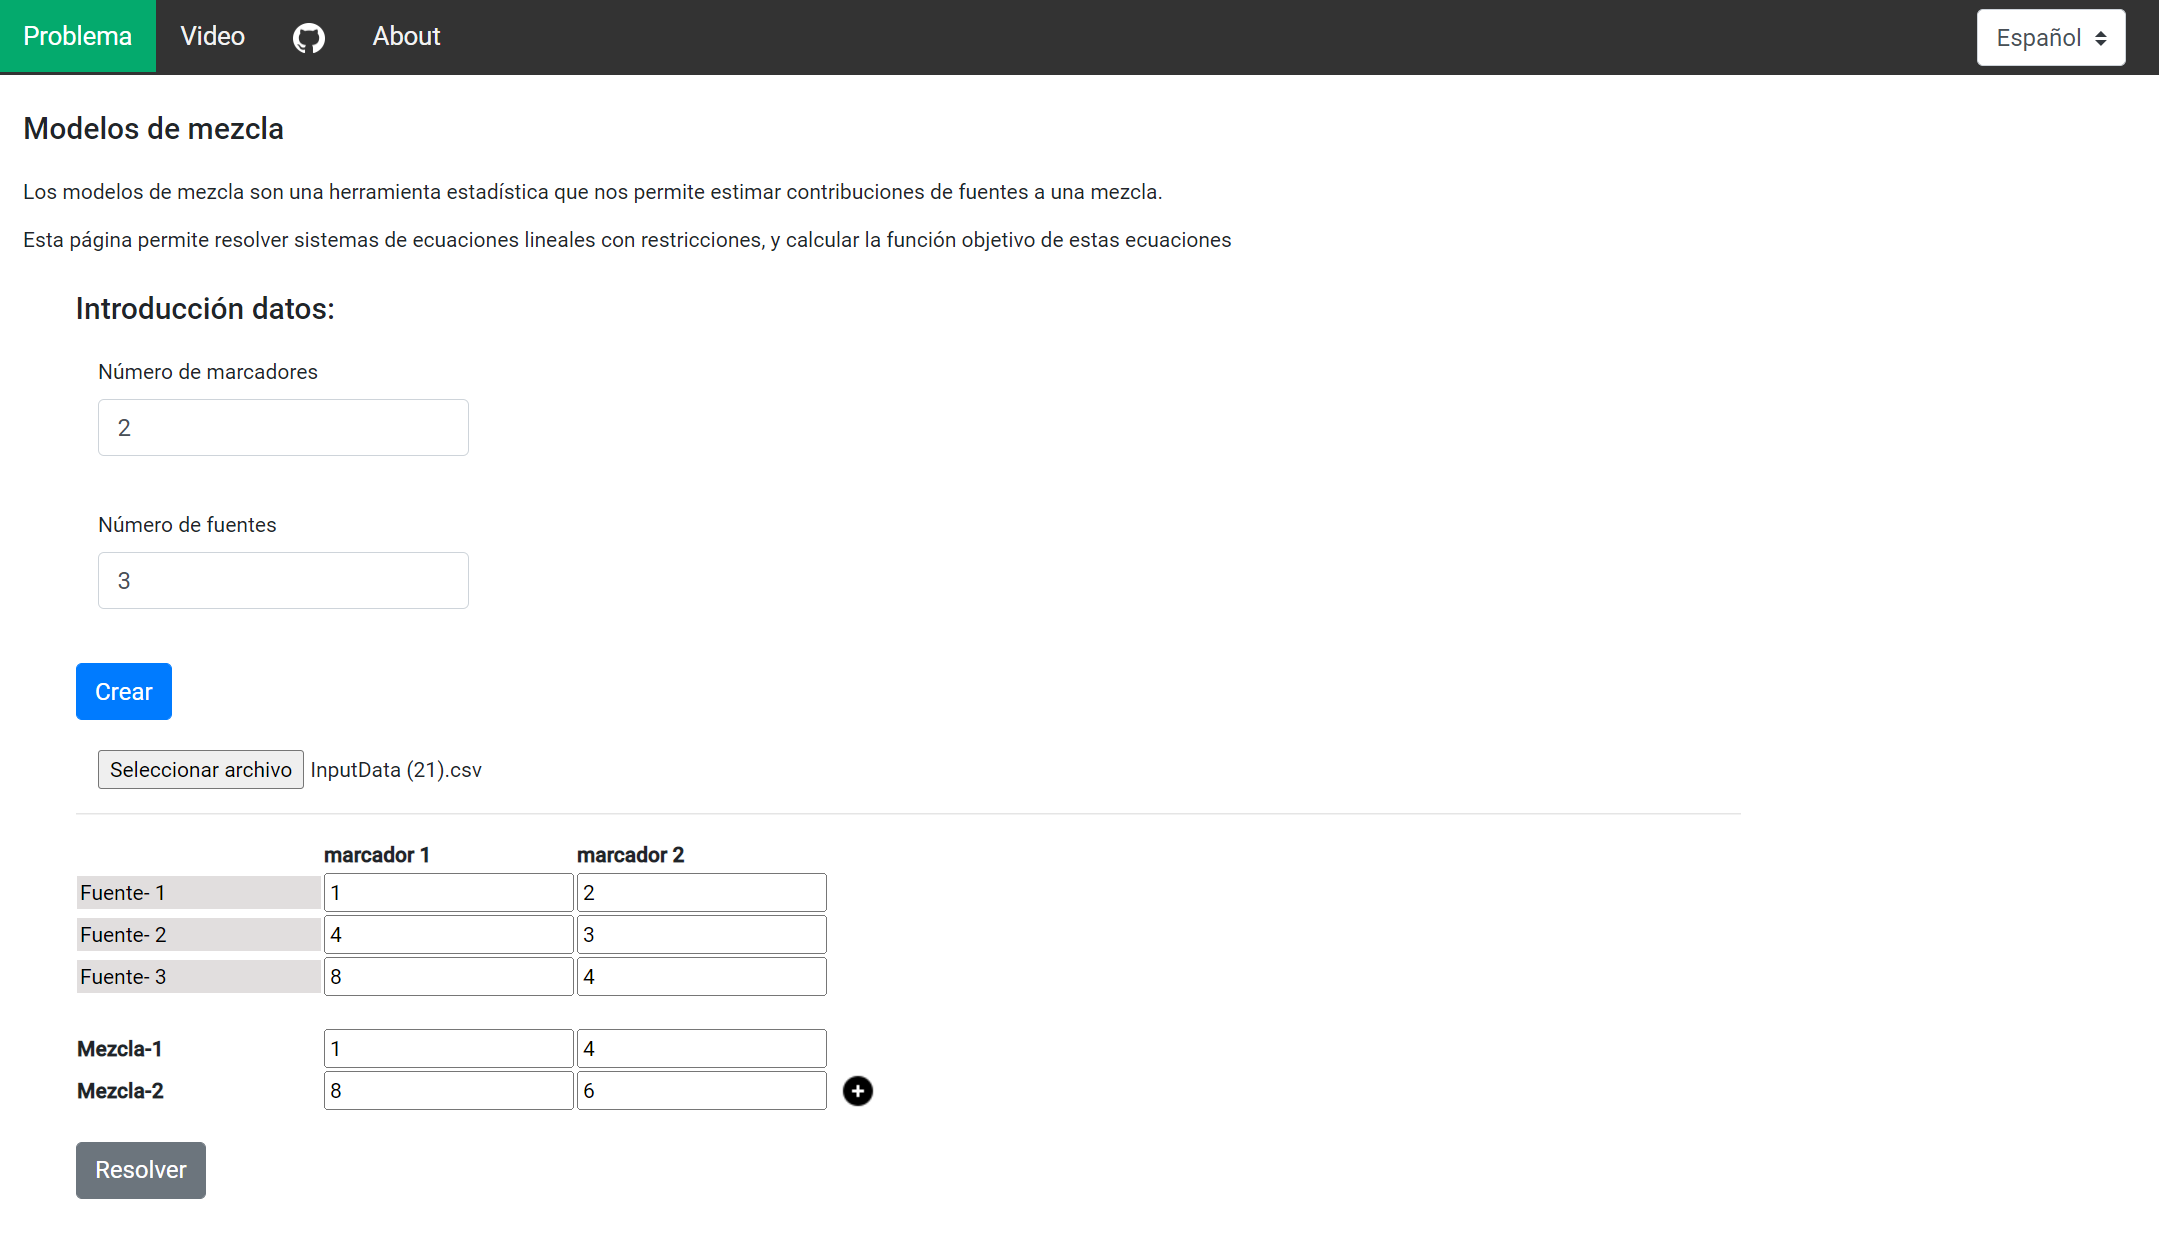
\includegraphics[width=1\textwidth]{img/importVisual.PNG}
\caption{Importar visual web}
\label{fig:visualwebimport}
\end{figure}